\chapter{Proceso de desarrollo}
\epigraph{How does a project get to be a year late?... One day at a time.}%
{Fred Brooks}

A esta altura ya hemos presentado los principales conceptos biol\'ogicos
involucrados en este trabajo, el dise\~no de vacunas atenuadas y la
formalizaci\'on del problema que nos propusimos resolver. En los cap\'itulos
restantes veremos los aspectos t\'ecnicos m\'as relevantes sobre el desarrollo
del software.

\section{Modelo de desarrollo}

Para llevar adelante el desarrollo del software, se opt\'o por el cl\'asico
modelo de cascada. Fundamentalmente debido a su simplicidad y a que los
requerimientos con que deb\'ia cumplir el software estaban bien definidos desde
el inicio, no solo a nivel funcional, sino tambi\'en en cuanto a principios del
dise\~no orientado a objetos.

\subsection{Etapas de la cascada}

Las etapas que se llevaron a cabo durante el desarrollo de este trabajo y que
veremos con mayor detenimiento en los siguientes cap\'itulos, fueron las
siguientes:
\begin{enumerate}
 \item Especificaci\'on de requerimientos.
 \item Dise\~no.
 \item Implementaci\'on.
 \item Verificaci\'on.
\end{enumerate}

Quedaron fuera del alcance las etapas ``Instalaci\'on'' y, por supuesto,
``Mantenimiento''.

\subsection{Consideraciones del modelo}

Para implementar el modelo de cascada se tuvieron en cuenta algunas
consideraciones con respecto al contexto en el que se desarroll\'o el software
y que veremos a continuaci\'on. 

Por un lado, todas las etapas que enumeramos m\'as arriba deb\'ian ser llevadas
a cabo por la misma persona. Esto es significativamente distinto a contar con
grupos de personas o equipos independientes para cada etapa y en donde la
documentaci\'on generada en cada fase es fundamental para la comunicaci\'on
entre los distintos equipos. En este sentido, usamos un modelo de cascada con
``solapamiento'', tambi\'en conocido como \textit{Sashimi}\cite{Mcconnell96},
que permite empezar una etapa sin haber terminado por completo la anterior.
Debido a que en este modelo es m\'as natural la continuidad del personal entre
las distintas etapas, no es necesario generar tanta documentaci\'on como en el
modelo de cascada ``puro'' y esto agiliz\'o el proceso de desarrollo.

Por otro lado, el rol de ``cliente'' en el proceso de desarrollo fue cubierto
por miembros de \ac{FuDePAN} que garantizaron el conocimiento del dominio de
manera tal de poder realizar la ``Especificaci\'on de requerimientos'' pero al
mismo tiempo, contaban con los conocimientos t\'ecnicos de dise\~no y
programaci\'on orientada a objetos como para supervisar el desarrollo en estos
aspectos. En este sentido, se tomaron algunos elementos de la variante al modelo
de cascada ``puro'' que se conoce como \textit{Staged
Delivery}\cite{Mcconnell96} o ``implementaci\'on incremental'' que nos
permitieron realizar revisiones peri\'odicas con miembros de \ac{FuDePAN}
durante las etapas de ``Dise\~no'' e ``Implementaci\'on''.

En la Figura~\ref{modelos} se pueden ver el modelo de cascada ``puro'' y las
variantes descriptas anteriormente y que adoptamos para este trabajo.

\begin{figure}
 \centering
  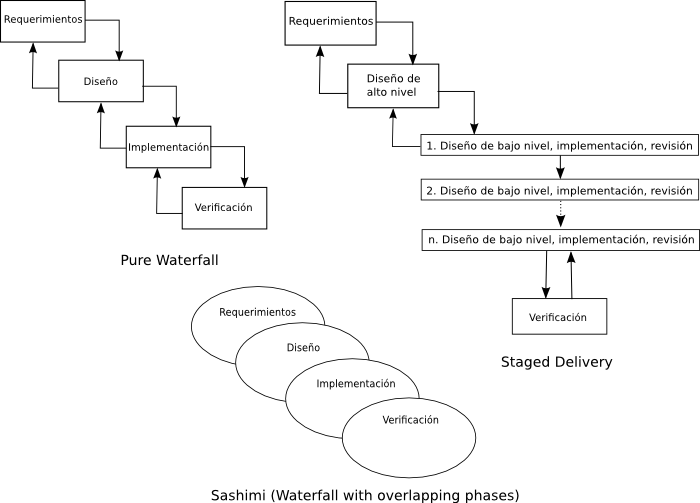
\includegraphics[scale=0.6]{modelos}
  \caption{Modelos de desarrollo}
  \label{modelos}
\end{figure}


Por \'ultimo, con el fin de validar los requerimientos del software que se
consideraban m\'as importantes, durante la etapa de ``Dise\~no'', se
implement\'o un prototipo utilizando el lenguaje de programaci\'on Python.

\section{Ecosistema}

El ``ecosistema'' de herramientas que se utilizaron para llevar adelante el
proceso de desarrollo son las siguientes:

\begin{itemize}
 \item \textbf{Lenguaje de programaci\'on:} El software se implement\'o en
\textbf{C++}\footnote{\url{http://cplusplus.com}}.
 \item \textbf{Lenguaje de dise\~no:} El dise\~no del software se hizo
utilizando \textbf{UML}\footnote{\url{http://www.uml.org}}.
 \item \textbf{Control de versiones:} Se utiliz\'o el sistema de control de
versiones \ac{SVN}\footnote{\url{http://subversion.apache.org}} y puede ser
consultado en \url{http://vac-o.googlecode.com}.
 \item \textbf{Sistema de ``construcci\'on'':} Para automatizar el
proceso de compilaci\'on del c\'odigo fuente se
utiliz\'o \textbf{CMake}\footnote{\url{http://www.cmake.org}}.
 \item \textbf{Automatizaci\'on de pruebas:} Para realizar la verificaci\'on del
software, se opt\'o por implementar pruebas unitarias utilizando
\textbf{google-test}\footnote{\url{http://googletest.googlecode.com}} y
\textbf{google-mock}\footnote{\url{http://googlemock.googlecode.com}}. 
 \item \textbf{An\'alisis est\'atico:} Se utilizaron las herramientas
\textbf{astyle}\footnote{\url{http://astyle.sourceforge.net}} y
\textbf{cppcheck}\footnote{
\url{http://sourceforge.net/apps/mediawiki/cppcheck}}.
 \item \textbf{An\'alisis din\'amico:} Se utilizaron las herramientas
\textbf{valgrind}\footnote{\url{http://valgrind.org}} y
\textbf{gcov}\footnote{\url{http://gcc.gnu.org/onlinedocs/gcc/Gcov.html}} para
verificar la ausencia de ``memory leaks'' y la cobertura de las pruebas.
\end{itemize}
